\documentclass[10pt,twocolumn,letterpaper]{article}

\usepackage{cvpr}
\usepackage{times}
\usepackage{epsfig}
\usepackage{graphicx}
\usepackage{amsmath}
\usepackage{amssymb}
\usepackage{mathtools}
\usepackage{array}
\usepackage{multirow}

% Box for the confusion matrix
\newcommand\MyBox[2]{
	\fbox{\lower0.75cm
		\vbox to 1.7cm{\vfil
			\hbox to 1.7cm{\hfil\parbox{1.1cm}{#1#2}\hfil}
			\vfil}%
	}%
}


% Include other packages here, before hyperref.

% If you comment hyperref and then uncomment it, you should delete
% egpaper.aux before re-running latex.  (Or just hit 'q' on the first latex
% run, let it finish, and you should be clear).
\usepackage[breaklinks=true,bookmarks=false]{hyperref}

\cvprfinalcopy % *** Uncomment this line for the final submission

\def\cvprPaperID{****} % *** Enter the CVPR Paper ID here
\def\httilde{\mbox{\tt\raisebox{-.5ex}{\symbol{126}}}}


% Pages are numbered in submission mode, and unnumbered in camera-ready
%\ifcvprfinal\pagestyle{empty}\fi
\setcounter{page}{1}
\begin{document}

%%%%%%%%% TITLE
\title{Assignment 1, Deep Learning Fundamentals, 2020 \\ Perceptron implementation and testing on the Pima Diabetes dataset}

\author{Julian Cabezas Pena\\
University of Adelaide, student ID: a1785086\\
SA 5005 Australia\\
{\tt\small julian.cabezaspena@student.adelaide.edu.au}
% For a paper whose authors are all at the same institution,
% omit the following lines up until the closing ``}''.
% Additional authors and addresses can be added with ``\and'',
% just like the second author.
% To save space, use either the email address or home page, not both
}

\maketitle
%\thispagestyle{empty}

%%%%%%%%% ABSTRACT
\begin{abstract}
Classification Machine Learning algorithms take an input vector and classify it in discrete classes. One of the first classifications algorithms to be invented, and one of the simplest neural networks, is the Perceptron, that deals with binary classification problems by adjusting a set of weights to find an optimum hyperplane to separate the classes. 

In this research, a classic single-layer Perceptron algorithm was implemented to create a diabetes classification model based on patient data, using the Pima Indians diabetes dataset. Moreover, the single-layer Perceptron was improved by adding a hidden layer, using sigmoid functions and implementing a back propagation algorithm to train the weights. The results of these algorithms were compared with the Support Vector Machine (SVM) and Random Forest (RF) model performances. This comparison yielded that the SVM outperformed all the other method (overall accuracy=0.7857), being followed by the multi-layer Perceptron (overall accuracy=0.7532), although the latter detected slightly more True Positives, a fact that can be relevant in the context of disease prediction. The inclusion of an extra layer in the Perceptron algorithm increased its performance, showing that, in this case, a complexity increase in the neural network can produce better classification performance.
\end{abstract}

%%%%%%%%% BODY TEXT
\section{Introduction}

In the field of pattern recognition and machine learning, classification problems are one of the most common tasks. In these kind of problems, an algorithm takes a vector $X$ as input, and assigns it to one or many $K$ discrete classes \cite{Bishop2006}. Considering that the labelled data take values in a discrete set, the input space can be divided in regions that can be labelled according to the classification. Boundaries of these regions can be smooth or rough, depending on the function applied by the algorithm \cite{Hastie2009}. When lineal functions are used to estimate these decision boundaries or surfaces, these algorithms can be labelled as part of the "linear models for classification" family, while data sets whose classes can be separated by lineal functions, are often called to be lineally separable \cite{Bishop2006}

The Perceptron algorithm is one of the first linear models for classification, introduced by Rosenblatt \cite{Rosenblatt1957}, is often considered one of the first neural networks. The Perceptron deals with binary (two class) classification problems \cite{Bishop2006}, by adjusting a set of weights to find a separating hyperplane in the training data, by minimizing the distance of misclassified data to the decision surface or boundary \cite{Hastie2009}.

In the field of classification problems, the diagnosis or determination of he risk of diseases based on clinical data is a recurrent field of study. These classification algorithms can help decision makers to predict the patient outcome based on the patient data \cite{Bellazzi2008}, making appropriate and well-timed decisions. One of the diseases that has been extensively researched in this field is the Diabetes Mellitus (DM); this chronic condition is characterized by high levels of glucose in the blood, caused either by the failure of the pancreas to produce enough insulin or the inefficiency of the body to efficiently use it \cite{Wu2018}. 

The objective of this research is to implement the Perceptron algorithm and to test if it can effectively predict the Diabetes Mellitus disease based on patient data, using the PIMA diabetes dataset. Additionally, the inclusion of a hidden layer to implement a multi-layer Perceptron (MLP) is proposed to be tested. Finally, this research aims to compare the single layer and multi-layer Perceptron performances against other machine learning algorithms, such as Support Vector Machines (SVM) and Random Forest (RF).

%-------------------------------------------------------------------------

\section{Related work}


The prediction of medical diseases is one of the fields where different machine learning methods have been extensively tested, with a special emphasis on the prediction of Diabetes Mellitus, where several models have been implemented \cite{Xu2017,Ahmad2013,Santhanam2015,Wu2018}, as an early diagnosis of the disease can be beneficial for the patient.

Multiple machine learning methods can be found in the literature on the prediction of Diabetes Mellitus. As an example, Santhanam \& Padmavathi \cite{Santhanam2015} used K-means and genetic algorithms to reduce the dimension of the dataset to integrate it into a Support Vector Machine(SVM) algorithm, archiving 96.71\% accuracy in the PIMA Indians Diabetes dataset; while Ahmad et al \cite{Ahmad2013} used a hybrid Genetic Algorithm together with a multi-layer Perceptron to archive 80.4\% accuracy o the same dataset.

Using a different dataset from the University of Virginia, Xu et al \cite{Xu2017} used a random forest model to predict the risk of Diabetes Mellitus based on readily available indicators (age, waist, weight etc), archiving 84.13\% of accuracy when sufficient data is provided.


\section{Methods}

\subsection{Pima Indian Diabetes Dataset}

The Pima Indian Diabetes dataset consists in the information of 768 patients from a population close to Phoenix, Arizona, USA \cite{Wu2018}; all of the patients are woman over the age 21 \cite{Xu2017} belonging to the Pima indiginous community. In this dataset, 268 (34.9\%) of the patients tested positive for Diabetes Mellitus (DM), while 500 (65.1\%) tested negative. Each row of data contains 8 attributes \cite{Wu2018}, apart from the classes label (Positive DM or Negative DM):

\begin{itemize}
	\item Number of pregnancies
	\item Glucose concentration in a oral tolerance test
	\item Skin fold thickness in the triceps
	\item Body mass index (BMI)
	\item Serum insulin (2h)
	\item Diastolic blood pressure
	\item Diabetes pedigree function
	\item Age of the patient
\end{itemize}

\subsection{Data preprocessing}

When machine learning algorithms are applied, considerable performance problems in the predictions can be attributed to low data quality, especially in clinical data \cite{Installe2014}. Given this background, basic data preprocessing was applied to increase the performance of the models. Therefore, following the recommendations of Wu \textbf{et al} \cite{Wu2018}, it was noted that the features "Diastolic Blood Pressure" and "Body mass index (BMI)" presented zero values, that were interpreted as missing data, as the human body can not present these values. Thus, as in We \textbf{et al} \cite{Wu2018}, the zero values were replaced by the mean of the valid observations in these two variables. 
After the handling of these missing values, the dataset was scaled to have values between -1 and +1 in all the features, using a standard lineal transformation:

\begin{equation}
	x' = (b-a) \times \frac{x - min(x)}{max(x)-min(x)} + a
\end{equation}

where $b$ is the new maximum (in this case +1), $a$ in the new minimum (-1), $x$ is the original feature and $x'$ is the transformed feature.
The output label (the diabetes diagnosis) was also transformed to -1 (Negative DM) and +1 (Positive DM), to comply with the requirement of the Perceptron algorithm

\subsection{Single-layer Perceptron implementation}

The Perceptron is a a two class classifier that uses the input vector a set of weights $w$, over the input vector $x$ (Figure \ref{fig:perceptron}), that can be previously transformed \cite{Bishop2006} (as in this case). These elements are used to construct a linear model of the form:

\begin{equation}
	y(x,w) = f(w^T x)
\end{equation}

Then, a non-linear activation function is used to transform this numerical output $a$ into a discrete label using the following sign function \cite{Bishop2006}

\begin{equation}
f(a)= 
\begin{dcases}
+1,& \text{if } a\geq 0\\
-1,& \text{if } a< 0\\
\end{dcases}
\end{equation}


\begin{figure}[h]
	\begin{center}
		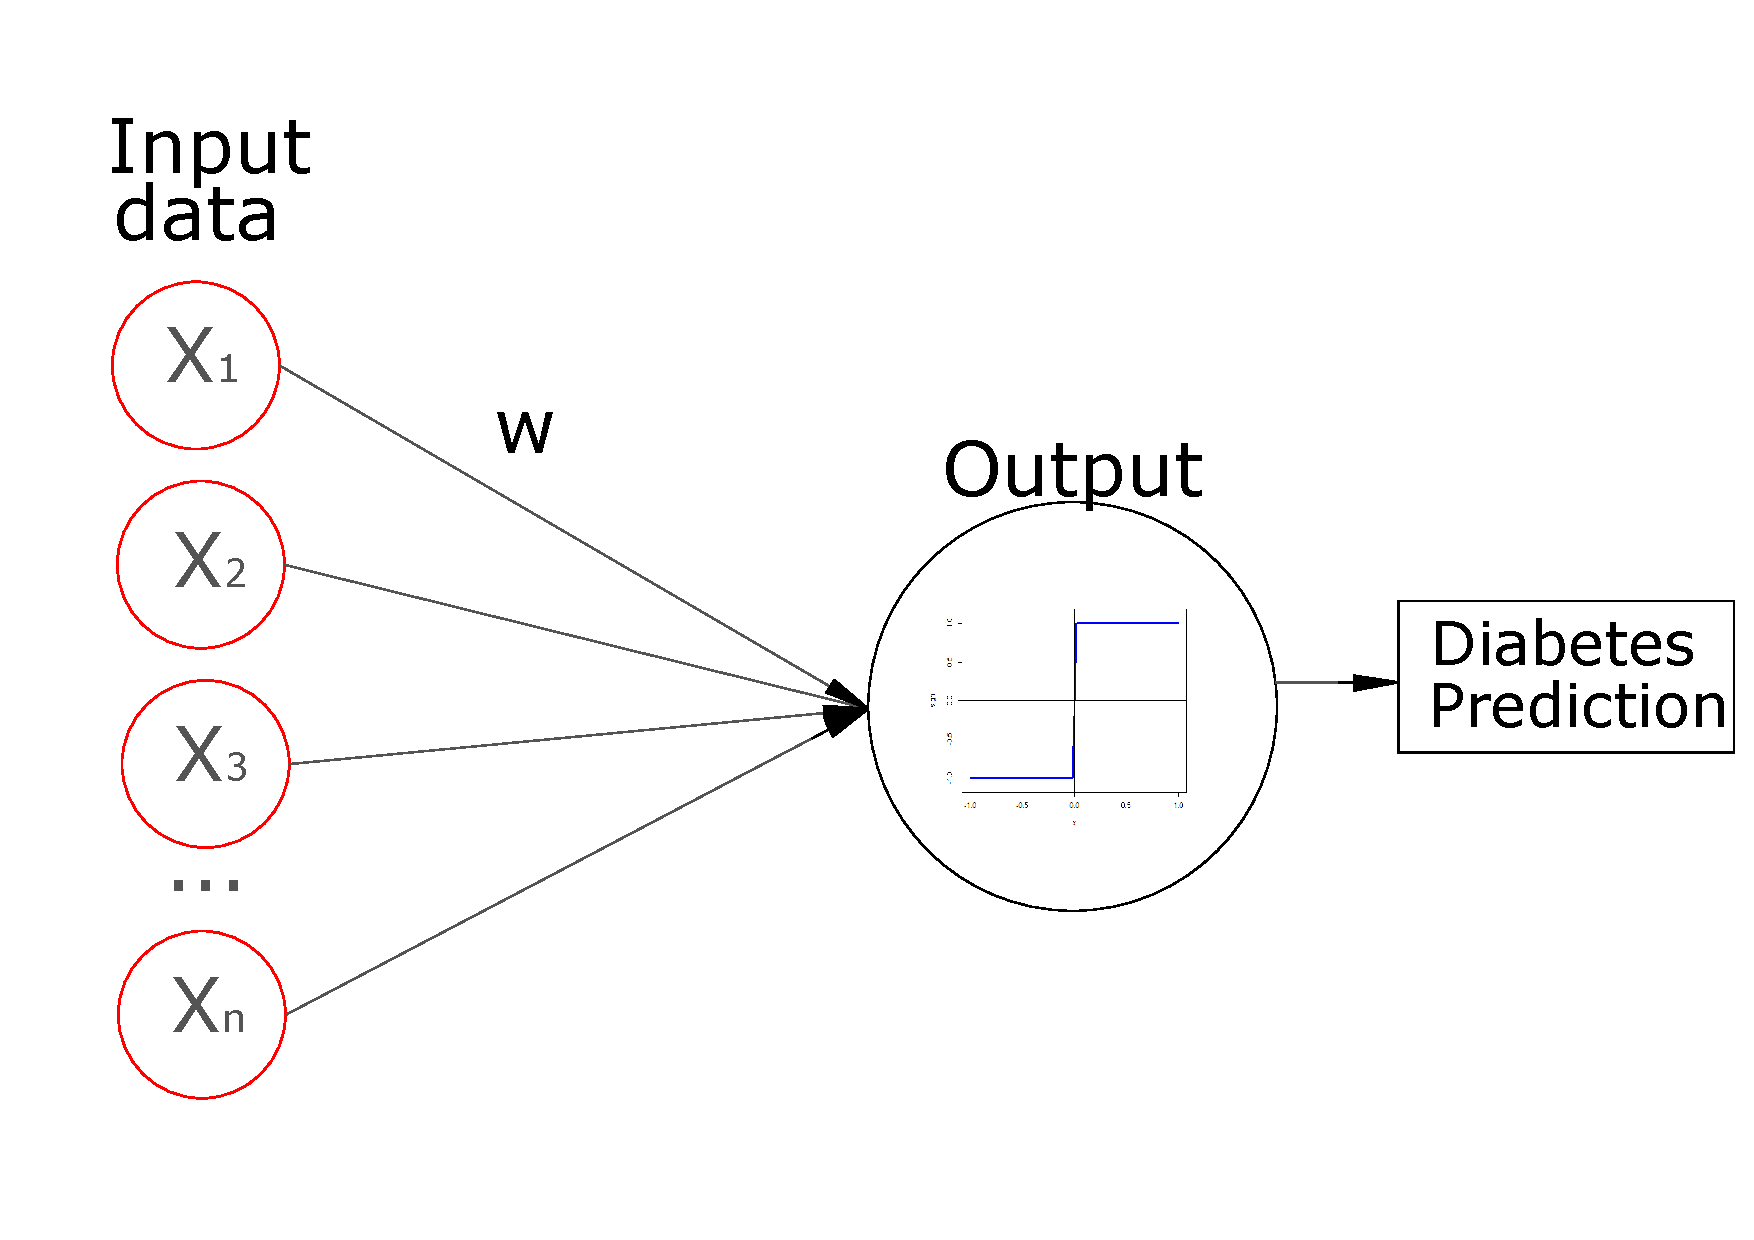
\includegraphics[width=1.0\linewidth]{Figura2.pdf}
	\end{center}
	\caption{Single layer Perceptron}
	\label{fig:perceptron}
\end{figure}


The weights of the Perceptron algorithm are iteratively trained using the following equations, that evaluates the predictions for each sample $i$ and compare it with the true label, using gradient descent to adjust the weights for each feature


\begin{equation}
	w_(t+1) = w_t + \eta \sum_{i=1}^{n} y_i x_i Error_i
\end{equation}

\begin{equation}
Error_i= 
\begin{dcases}
1,& \text{if } predicted_i \neq y_i\\
0,& \text{if } predicted_i = y_i\\
\end{dcases}
\end{equation}

Where $w$ is the vector of weights, $y_i$ are true label in the dataset and $x_i$ is the input value of the feature

In this case, the initial weights ($w$) were generated using random numbers coming from a normal distribution of mean = 0 and standard deviation = 0.1

In order to account for the bias term \cite{Vapnik1995}, a new column in the input data was filled by ones (1.0), and treated as any other variable.

According to Ripley \cite{Ripley1996}, the Perceptron algorithm will perform poorly in the case of a non linearly separable dataset, as optimizing the number of error made by this algorithm is hard. Also, in nonlinear separable problem, this algorithm may not converge in a fixed set of weights, being dependent in the number of iterations in the training.  

\subsection{Multi-layer Perceptron implementation}

In order to improve the single layer Perceptron, a hidden layer with a variable number of layers  was implemented in between the Output and the Input layer. Also, in order to reflect non linear boundaries \cite{Vapnik1995}, a sigmoid function of the following form was used to activate the hidden and output layer:

\begin{equation}
sigmoid(x) = \frac{1}{1-e^{-x}}
\end{equation}

As showed in Figure \ref{fig:mlp}, the multi-layer Perceptron the input data ($x$) feed the hidden layer nodes by appling a $w1$ set of weights, just as in the single layer perceptron, then, these hidden layer nodes are activated with the above mentioned sigmoid equation, feeding the output layer though the application of the $w2$ set of weights. This output layer is also activated by a sigmoid function. Finally, the diabetes prediction is determined by a threshold of 0.5 in the final output, as the sigmoid function generates values from 0 to 1. Considering this particularity, for this specific case, the label values were encoded as 1: Positive DM and 0: Negative DM.

\begin{figure}[h]
	\begin{center}
		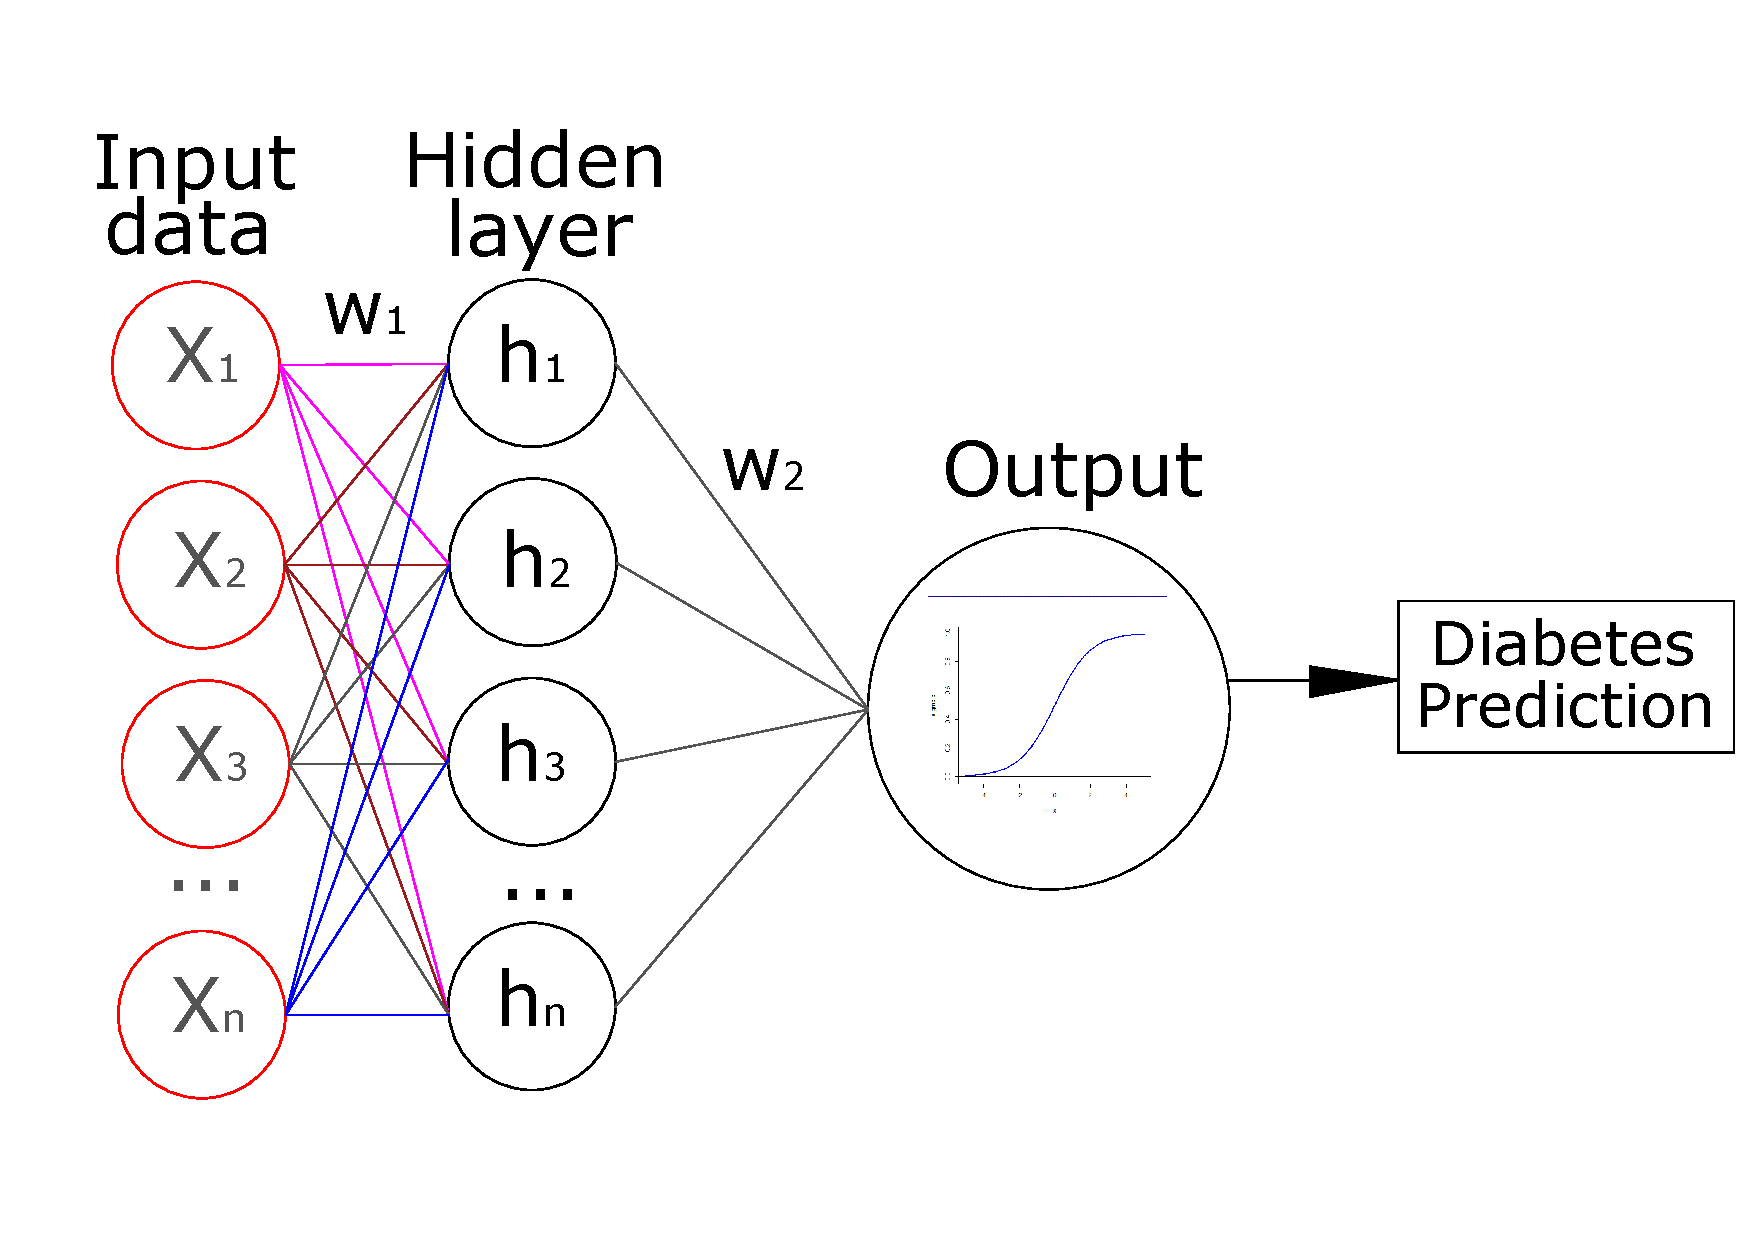
\includegraphics[width=1.0\linewidth]{Figura.pdf}
	\end{center}
	\caption{Multi-layer Perceptron}
	\label{fig:mlp}
\end{figure}


In this case, the algorithm has two sets of weights ($w1, w2$), the first one correspons to a matrix of dimensions $[number of features, number of hidden layer nodes]$, while $w2$ is a vector of length equal to the number of hidden layer nodes. As explained by Vapnik \cite{Vapnik1995}, in order to train them, a iterative back-propagation workflow has to be implemented, consisting in three steps

(i) Forward pass

Firstly, each hidden layer node is activated using the sigmoid function, getting the values from the input values multiplied by the set of $w1$ weights corresponding to the hidden layer $h_i$

\begin{equation}
h_i(x,w1) = S(w1_i^T x)
\end{equation}

Then the output layer is activated using the input from the hidden layers, by multiplying the hidden post activation values with the second set of weights ($w2$)

\begin{equation}
o(h,w2) = S(w2^T h)
\end{equation}

(ii) Backward pass

The backward pass computes the error in the output layer and then passes those values to the previous layer, in this case the hidden layer

\begin{equation}
b(output) = o(h,w2) - y_i
\end{equation}

\begin{equation}
b_i(hidden) = b(output) \nabla S(w2^T h)*x2_i
\end{equation}

iii) Weight update

In order to update the weights, a step real positive value($\eta$) is defined, and the backward passes of the respective layers are used to update each set of weights

\begin{equation}
w1_i(t+1) = w1_i(t) - \eta \sum_{i=1}^{n} b_i(hidden) x_i w1_i \nabla S(w1^T x_i)
\end{equation}

\begin{equation}
w2_i(t+1) = w1_i(t) - \eta \sum_{i=1}^{n} b_i(output) h_i w2_i \nabla S(w2^T h_i)
\end{equation}

Just as in the single-layer perceptron, a bias term was included by inserting a column of "ones" (1.0) in the input matrix

\subsection{Performance metrics}

The dataset under study corresponds to an unbalanced dataset (there is much more negative DM than positive DM), and as such, some considerations have to be made in order to correctly compare methods and asses the performance of the models \cite{Hoens2013}. Therefore, two different metrics were used for comparison

\textbf{Accuracy}: Although this metric can be misleading in the case of unbalanced datasets, it is the most commonly used metric \cite{Hoens2013} and can help compare the overall performance of the method:

\begin{equation}
accuracy = \frac{TP+TN}{TP+FP+TN+FN}
\end{equation}

where $TP$ is the number of true positive, $TP$: true negative, $FP$: false positives and $FN$: false negatives.

In order to use a metric than can asses the performance in this unbalanced problem, the F1 score was used, as it balances the precision and recall of the algorithm, being a metric that has useful properties in unbalanced cases \cite{Hoens2013}

\begin{equation}
precision = \frac{TP}{TP+FP}
\end{equation}

\begin{equation}
recall = \frac{TP}{TP+FN}
\end{equation}

\begin{equation}
F1 = 2 \frac{precision * recall}{precision + recall}
\end{equation}

\subsection{Training, parameter tuning and testing}

In order to obtain the best possible model to predict the occurrence of Diabetes Mellitus (DM) in future data, the complete dataset was partitioned into training (80\%) and testing data (20\%), as the data is imbalanced (it contains 34.9\% of samples with positive DM), a stratified sampling was used to ensure that this proportion is approximately maintained in the training and testing data. 

The single-layer Perceptron presents two parameters that can impact the performance of the model: the step value and the number of iterations (epochs) in the training. In order to pick the best possible values, a grid search was implemented. Therefore, the training data was split into 4 groups using stratified sampling to maintain the proportion of positive and negative labels. Then 4-fold cross validation was used to test all the possible combinations of values for these parameters in the following vectors: $step = (0.1,0.2,0.3...1.0)$ and $n_\mathrm{iterations} = (10,20,30...100)$

In each of the parameter combinations, the F1 index was calculated in order to asses the performance of the model, and the obtained values were averaged between the 4-fold operations, giving a mean F1 value for each combination of parameters. Once all the possible combinations of parameter values were tested, the set of parameters with the biggest F1 score was picked. These parameters were used to  where the above mentioned metrics were calculated to asses the model performance.

In the case of the multi-layer Perceptron, the parameter tuning also included the testing of different number of nodes in the hidden layer, thus, in this case, the grid search included the following vectors: $step = (0.1,0.3,0.5,0.7,0.9,1.1)$, $n_\mathrm{iterations} = (10,30,50,70,90,110)$ and $nodes_\mathrm{hidden layer} = (3,4,5)$

\subsection{Comparison with other machine learning methods}

In order to asses the performance of the Perceptron algorithms against other well-established machine learning models, a Random Forest classifier and a Support Vector Machine model were tested to predict Diabetes Mellitus (DM), as these models are present in the related literature \cite{Xu2017,Santhanam2015}, using the same pre-processing steps and score metrics than those used in the Perceptron implementations

\textbf{Random Forest}: This bagging method was first introduced by Breiman \cite{Breiman2001b}, and consists in the a large collection of de-correlated decision trees, using a user-defined number of trees ($n_\mathrm{trees}$), the algorithm draws a bootstrap sample of the training data, to grow a decision tree of the subset data, selecting a random number of variables in each split ($max_\mathrm{features}$), to then determine the best split point among the drawn variables, generating two child nodes. After all the trees are grown ()forming a \emph{Random Forest}), new testing data can be predicted by obtaining a class vote from each decision tree in the forest, and then classifying it using majority vote \cite{Hastie2009}.

According to Hastie \cite{Hastie2009}, Random Forest algorithms can perform remarkably well with very little tuning, while Breiman \cite{Breiman2001b} claims that their results can be highly interpretable. Moreover, this model is quite robust in the presence of noisy variables, but can perform poorly with a small $max_\mathrm{features}$ \cite{Breiman2001b}

In this case, the tuned parameters using were the maximum number of features in each split($max_\mathrm{features}$), and the number of trees ($n_\mathrm{trees}$). Thus, the vectors for the grid search were: $max_\mathrm{features} = (1,2,3...8)$ and $n_\mathrm{trees} = (100,300,500...2100)$, that were tested using cross-validation (as described in the previous section)

\textbf{Support Vector Machine}: This supervised classification algorithm was developed by Vapnik \cite{Vapnik1995}, and consist in an hyperplane that separates a high dimensional space defined by the input variables into discrete classes. This hyperplane is defined to have the largest possible distances to the closest point of either class \cite{Hastie2009}, thus, maximizing the margin ($M$) between two classes. 

\begin{equation}
Max \: M \:\:\:\: constrained \:\:by  \:\: y_1(x_i^T \theta + \theta_0) \geq M
\end{equation}

This algorithm can define an hyperplane even when classes overlap (non linearly separable), maximizing the margin but allowing some points to be in the wrong side of the boundary, defining the slack variables $xi_i$, thus, the margin constrain for defining the hyperplane can be modified as \cite{Hastie2009}

\begin{equation}
y_1(x_i^T \theta + \theta_0) \geq M(1-\xi_i) 
\end{equation}

if $M$ is redefined as $M = 1/||\theta||$, we can write the previous equation as \cite{Hastie2009}:

\begin{equation}
min \frac{1}{2}||\theta||^2 + C \sum^n_{i=1}\xi_i
\end{equation}

This equation can be then solved using Lagrange multipliers \cite{Hastie2009}

\begin{multline}
L_p = \frac{1}{2}||\theta||^2 + C \sum^n_{i=1}\xi_i - \sum^n_{i=1}\alpha_i[y_1(x_i^T \theta + \theta_0) - (1-\xi_i)] \\ - \sum^n_{i=1}\mu_i\xi_i
\end{multline}

Although this algorithm initially use lineal boundaries between the different classes, it can be defined by other kinds of boundaries form, using a "kernel trick" (more details in Hastie \cite{Hastie2009})

Support vector machine are widely used in the medical sciences, and can perform greatly in image classification and other pattern recognition tasks. Although some practitioners have criticized SVM method for being difficult to interpret and explain. This kind of method is commonly compared with neural networks, as both use sigmoid functions and the finding of optimal hyperplanes \cite{Bell2014}

In this case, the tuning parameters were the cost and the type of kernel, that were tested in the cross validation stage using grid search with $cost = (0.5,1.0,1.5...10)$ and $kernel = (linear, polynomial, radial, sigmoid))$. 

\section{Code}

The code, along with the requirements and setup instructions for the reproduction of the above-mentioned method, can be found in the following GitHub repository: \url{https://github.com/juliancabezas/deep_learning_perceptron} 

\section{Results and experimental analysis}

\subsection{Parameter tuning}

The k-fold testing of different parameters gave the result of Table \ref{table:tuning}, where it is possible to see that the RF shows a better F1 score using the maximum number of trees that was trained, and 4 as maximum number of features (half of the dataset). On the other hand, the single layer and the multi-layer Perceptron show similar performances (0.6539 and 0.6377 respectively), with the single layer Perceptron showing the best performance with 20 iterations to train the weights, while the multi-layer Perceptron shows 70, as the procedure to train them is more complex. Finally, the best performance of the Support Vector Machine (SVM) model was archived with a lineal kernel an a cost of 3.0.

\begin{table}[h]
	\begin{center}
		\begin{tabular}{|p{1.6cm}|p{4.3cm}|p{1cm}|}
			\hline
			Algorithm & Tuned parameters & F1 \\
			\hline\hline
			Perceptron & $n_\mathrm{iter} = 100$ \& $step = 0.7$ & 0.6539 \\
			MLP & $n_\mathrm{iter} = 90$, $step = 0.3$ \& $nodes_\mathrm{hidden} = 4$ & 0.6507 \\
			SVM & $cost = 3.0$ \& $kernel = linear$ & 0.6377 \\
			RF & $max_\mathrm{features} = 4$ \& $n_\mathrm{trees} = 1100$ & 0.6751 \\
			\hline
		\end{tabular}
	\end{center}
	\caption{Parameter tuning (MLP = Multi-Layer Peceptron, SVM = Support Vector Machine, RF = Random Forest)}
	\label{table:tuning}
\end{table}


\subsection{Model testing}

The results of the application of the different models in the test dataset \ref{table:tuning} show that the best results in terms of the F1 score, that generates a compromise between recall and precision, are presented in the multi-layer Perceptron (0.6731 against 0.6484 in the single-layer Perceptron and the SVM models). While comparing the accuracy, the Support Vector Model (SVM) (accuracy = 0.7857) clearly outperforms the single-layer Perceptron models and the Random Forest (RF) model, while being only slightly superior to the multi-layer perceptron (0.7792), that shows a better F1 score, generating an more balanced model. The poor accuracy of the single layer Perceptron, that is just slightly poorer that the trivial solution (classifying all samples as negative DM), can be attributed to the fact that the data is non linearly separable \cite{Ripley1996}

Regarding the Perceptron models, the inclusion of the hidden layer containing 4 nodes and the use of the sigmoid function to activate them generates significant improvements in the accuracy (0.6623 to 0.7792) and F1 score (0.6486 to 0.6731), showing that in this case, increasing the complexity of the neural network can be beneficial for its prediction capacity

\begin{table}[h]
	\begin{center}
		\begin{tabular}{|p{1.8cm}|p{1.5cm}|p{1.5cm}|}
			\hline
			Algorithm & F1 & Accuracy \\
			\hline\hline
			Perceptron & 0.6486 & 0.6623 \\
			MLP & 0.6731 & 0.7792 \\
			SVM & 0.6451 & 0.7857 \\
			RF & 0.6111 & 0.7272 \\
			\hline
		\end{tabular}
	\end{center}
	\caption{Model performance in the test data (MLP = Multi-Layer Perceptron, SVM = Support Vector Machine, RF = Random Forest)}
	\label{table:testing}
\end{table}

We can determine, by looking at the maximum values in the F1 and accuracy indicators, that the two best performing models are the MLP and the SVM, with the SVM obtaining an accuracy less than 1\% greater than what was obtained by the MLP. Although, when looking at the details of the confusion matrix of these two algorithms, the SVN appears to detect a great percentage of the negative cases (91\%), while  missing a significant number of positive cases (44\%) (Figure \ref{fig:cmsvm}). In the case of the diagnosis of diseases, this consideration can have a great impact in the utility of the model, preventing the decision makers to perform early diagnosis of this disease.

\begin{figure}[h]
\noindent
\renewcommand\arraystretch{1.5}
\setlength\tabcolsep{0pt}
\begin{tabular}{c >{\bfseries}r @{\hspace{0.7em}}c @{\hspace{0.4em}}c @{\hspace{0.7em}}l}
	\multirow{10}{*}{\rotatebox{90}{\parbox{1.1cm}{\bfseries\centering Label value}}} & 
	& \multicolumn{2}{c}{\bfseries Prediction} & \\
	& & \bfseries Positive DM & \bfseries Negative DM & \bfseries Total \\
	& Pos. DM& \MyBox{TP=}{30} & \MyBox{FN=}{24} & 54 \\[2.4em]
	& Neg. DM& \MyBox{FP=}{9} & \MyBox{TN=}{91} & 100 \\
	& Total & 39 & 115 & 154
\end{tabular}
	\caption{Confusion matrix for the Support Vector Machine model}
\label{fig:cmsvm}
\end{figure}

On the other hand, the multi-layer Perceptron, although producing a lower overall accuracy, is able to detect a larger value of positive cases (65\%), but still missing  35\% of the positive cases (Figure \ref{fig:cmmlp}). This is reflected in the F1 score, where the MLP outperforms the SVM model.

\begin{figure}[h]
\noindent
\renewcommand\arraystretch{1.5}
\setlength\tabcolsep{0pt}
\begin{tabular}{c >{\bfseries}r @{\hspace{0.7em}}c @{\hspace{0.4em}}c @{\hspace{0.7em}}l}
	\multirow{10}{*}{\rotatebox{90}{\parbox{1.1cm}{\bfseries\centering Label value}}} & 
	& \multicolumn{2}{c}{\bfseries Prediction} & \\
	& & \bfseries Positive DM & \bfseries Negative DM & \bfseries Total \\
	& Pos. DM & \MyBox{TP=}{35} & \MyBox{FN=}{19} & 54 \\[2.4em]
	& Neg. DM & \MyBox{FP=}{15} & \MyBox{TN=}{85} & 100 \\
	& Total & 50 & 104 & 154

\end{tabular}
	\caption{Confusion matrix for the multi-layer Perceptron model}
\label{fig:cmmlp}
\end{figure}

These results indicate that neither of this models could be used in a medical environment, as could mislead the practitioners into missing the diagnosis of a potentially serious disease. 

Although the performance of the tested models was far from ideal (specially in the medical field), this research showed that the inclusion of a simple hidden layer can generate a simple multi-layer Perceptron model that outperformed more modern models as Random Forest, and can compete and generate more balanced results than well tested models as SVM. Giving the insight that the inclusion of more complexity in the model (more layer and/or nodes) could lead to a increased performance. Also, other more common activation functions (such as ReLU) could be used to improve the model \cite{Skansi2018}


\section{Conclusion}

The results of this experiment shows that the single-layer Perceptron, does not generate reliable results in the case of non-separable data, being outperformed by newer models such as Random Forest and SVM. The increase in performance of the Perceptron when adding an extra layer shows one of the main principles of deep neural networks, that benefit from the inclusion of multiple layers to solve non-linear and complex problems.

This research gave the insight that, although relative "classic" machine learning algorithms, such as Random Forest or Support Vector Machine, can be easy to implement, tune and interpret, relatively simple neural networks can easily compete with them, and that the more modern one will probably outperform them, showing that the future of machine learning will be seriously influenced by deep neural networks.

In future research, extra hidden layers, with different activation functions, can be tested to increase to generate a deeper multi-layer Perceptron, possibly increasing the  accuracy of the prediction, generating useful models for the medical community and taking advantage of modern computational power.


{\small
\bibliographystyle{ieee_fullname}
\bibliography{library}
}

\end{document}
